% Asset ID: A22StatisticalHypothesisTestingTikZ-001
% Source: Chapter 7 Hypothesis Testing Binomial transcript
% Related lesson section: Big Picture; Core Theory
% Purpose: Show the structure of a binomial hypothesis test.
% Related LO IDs: A22-HT-LO001, A22-HT-LO002, A22-HT-LO003

\documentclass[tikz,border=8pt]{standalone}
\usepackage{amsmath}
\usetikzlibrary{arrows.meta, positioning, decorations.pathreplacing}
\begin{document}
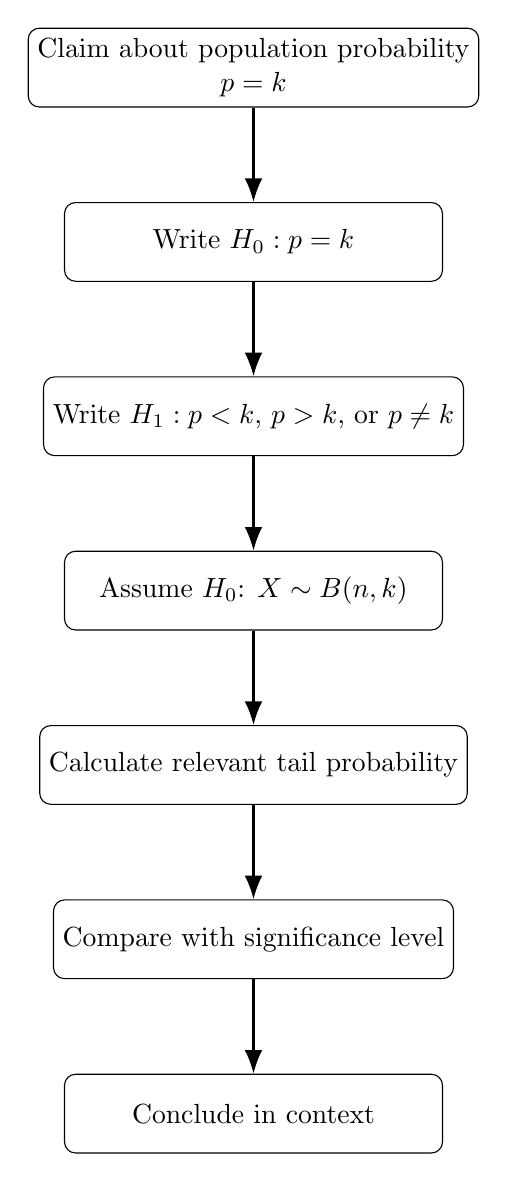
\begin{tikzpicture}[node distance=1.2cm, box/.style={draw, rounded corners, align=center, minimum width=4.8cm, minimum height=1.0cm}, arrow/.style={-{Latex[length=3mm]}, thick}]

\node[box] (claim) {Claim about population probability\\\(p=k\)};
\node[box, below=of claim] (h0) {Write \(H_0:p=k\)};
\node[box, below=of h0] (h1) {Write \(H_1:p<k\), \(p>k\), or \(p\ne k\)};
\node[box, below=of h1] (dist) {Assume \(H_0\): \(X\sim B(n,k)\)};
\node[box, below=of dist] (prob) {Calculate relevant tail probability};
\node[box, below=of prob] (decision) {Compare with significance level};
\node[box, below=of decision] (context) {Conclude in context};
\draw[arrow] (claim)--(h0);\draw[arrow](h0)--(h1);\draw[arrow](h1)--(dist);\draw[arrow](dist)--(prob);\draw[arrow](prob)--(decision);\draw[arrow](decision)--(context);

\end{tikzpicture}
\end{document}
